\chapter{Calculus Review}

This is part of the second lecture of the summer school series.

In linear algebra, we wanted to write all our information in the form of matrices. But linear algebra, restricts us to systems and functions to linear only. This assumption isn't always possible and hence, to represent other quantities such as polynomial path, a non linear curve on which we need to establish stability, we need to use non linear function. It is also important that we use something that the computer can use the non linear data, and with approximations among other things, get answers to our problems.

In general, if we have a function $f(x$, can we linearize it? If we could, then we could represent it in the matrix form

\section{Gradient}

Gradient can be defined as 

\begin{equation}
    f'(x) = \lim_{h \to 0} \frac{f(x+h) - f(x)}{h}
\end{equation}

But, this is single variable. If we have multiple variables, we can represent the gradient with respect to any of the variables.

\begin{equation}
    \frac{\partial f(x_1, x_2, ... x_n)}{\partial x_1} = \lim_{h_1 \to 0} \frac{f(x_1 + h, x_2, x_3, \cdots x_n) - f(x_1, x_2, \cdots x_n)}{h_1}
\end{equation}

Similarly, we can calculate the gradient for the remaining elements of x.

The slope is essentially the tangent to a curve. Hence, by taking a gradient, we are essentially linearizing by creating a line when we take derivative with a variable.

Here the input can be a vector, and let the function $f$ be one that gives us a scalar output. 

\begin{equation}
\nabla f =
\begin{bmatrix}
\frac{\partial f}{\partial x_1} \\
\frac{\partial f}{\partial x_2} \\
\vdots \\
\frac{\partial f}{\partial x_n}
\end{bmatrix}
\end{equation}

\href{https://atmos.washington.edu/~dennis/MatrixCalculus.pdf}{These notes} have a lot of examples of gradients involving matrices. Some of these questions were asked in the deep learning assignment. Computing derivatives of matrices is often unintuitive. In fact, even doing the math is tedious.

\section{Jacobian}

Now suppose that we have a function $f: R^N \to R^M$, takes a vector as input and produces a vector as output. Let the inputs be $\{ x_1, x_2, \cdots, x_n  \}$ and output be $\{ y_1, y_2, \cdots, y_m\}$. Then the derivative of $f$ at a point $x$, also called Jacobian is the $M \times N$ vector:

\begin{equation}
    J = \begin{bmatrix}
    \frac{\partial y_1}{\partial x_1} & \hdots & \frac{\partial y_1}{\partial x_n} \\
    \frac{\partial y_2}{\partial x_1} & \hdots & \frac{\partial y_2}{\partial x_n} \\
    \vdots & \ddots & \vdots \\
    \frac{\partial y_m}{\partial x_1} & \hdots & \frac{\partial y_m}{\partial x_n} \\
    \end{bmatrix}
\end{equation}

\subsection{Generalized Jacobian}

Just as a vector is a one-dimensional list of numbers and a matrix a two-dimensional grid of numbers, a tensor is a D-dimensional grid of numbers. Many operations in deep learning accept tensors as inputs and produce tensors as outputs. For instance, an image is usually represented as a three dimensional grid of numbers - height, width, and colour channels of the image. 

There is a lot of math here - nothing too fancy to understand. Refer to slides 12+ \href{https://github.com/RoboticsIIITH/summer-sessions-2020/blob/master/lecture-slides/deep_learning/vector_derivatives.pdf}{here}.

\textbf{There are some examples of derivatives \href{https://github.com/RoboticsIIITH/summer-sessions-2020/blob/master/lecture-slides/deep_learning/vector_derivatives.pdf}{here}}.

\section{Hessian}

Hessian of a function that is of the form $f: R^n \to R$, 

\begin{equation}
    \nabla^2 f = H = \begin{bmatrix}
    \frac{\partial^2 f}{\partial x_1^2} & \frac{\partial^2 f}{\partial x_1 \partial x_2} & \hdots & \frac{\partial^2 f}{\partial x_1 \partial x_n} \\
    \frac{\partial^2 f}{\partial x_1 \partial x_2} & \frac{\partial^2 f}{\partial x_2^2} & \hdots & \frac{\partial^2 f}{\partial x_2 \partial x_n} \\
    \vdots & \vdots & \ddots & \vdots \\
    \frac{\partial^2 f}{\partial x_1 \partial x_n} & \frac{\partial^2 f}{\partial x_2 \partial x_n} & \hdots & \frac{\partial^2 f}{\partial x_n^2} \\
    \end{bmatrix}
\end{equation}

This is a symmetric matrix.

\section{Model and Error}

How can we use the hessian and gradient? The reason for using this math is to model real data, and have some measure of quantities in the environment through sensors.

\begin{equation}
    X = f(P) \text{ in an ideal scenario}
\end{equation}

Now, we need to find parameters that can give the best result to measure the environment, or minimize the error. This function $f(P)$ need not be linear. This is where we need to use gradient and hessian.

\begin{equation}
    \norm{f(\hat{P}) - X} \text{ is to be minimized}
\end{equation}

\section{Linear Equations}

Sometimes, we can represent some sensors as linear models. We can use linear methods or decomposition methods to get a better reading from the model.

\begin{equation}
    f(P) = AP
\end{equation}

Here $A\; \epsilon R^{m \times n} \text{ and } P\; \epsilon R^n$. There are three cases:

\begin{itemize}
    \item $m < n$, we have many solutions. They form a vector space.
    \item $m = n$, we have either a unique solution or no solution.
    \item $m > n$, we have either a unique solution or no solution.
\end{itemize}

\textbf{No Solution case}

This happens when $b$ doesn't lie in the column space of A. If we don't have any solutions that are possible from the linear set of equations, we try to compute a vector that is close to the optimum.

\section{Non-Linear}

If we do not have a linear model, we need to find vector that fits the measurement data well.

\subsection{Taylor Series}

This is one approximation of a non linear function:

\begin{equation}
    f(x) = f(a) + \frac{f'(a)}{1!}(x-a) + \frac{f''(a)}{2!}(x-a)^2 + \frac{f'''(a)}{3!}(x-a)^3 + \cdots
\end{equation}

This is essentially a weighted sum.

If we have more variables, then we need to use a variant. We've already seen how we can use hessian and now for taylor series,

\begin{equation}
    f(x) = f(a) + \frac{\nabla f(a)^T}{1!}(x-a) + \frac{(x-a)^T \nabla^2f(a)(x-a)}{2!} +  \cdots
\end{equation}

Note that the transpose here is since they are all column vectors. By taking transpose, we can essentially take dot product. All the terms in the above expression are a vector, as opposed to the scalars in the single variate form. Most of the times, the first and second order approximation is enough. 

\begin{equation}
    Accuracy equations
\end{equation}

Using higher order estimations, only increase the accuracy of the estimate. 

\subsection{Cost Function}

We start with an initial estimate $P=P_0$ and we can use Taylor series to approximate cost function. We have an approximation of the cost at $P_0$. Now, we have a change of $\delta P$, then we can approximate cost of the new estimate.

\textbf{Most of this section is visited in detail in the SLAM: Optimization chapter.}

\subsubsection{First Order Method}

This method is called gradient descent. Now, if we take gradient with respect to parameter $P$, it is called Jacobian.

This is an iterative approximation and at every step, we decide what direction to take derivative in and how we can descent

\section{Contour line and Vector Field}

Now, if we take gradient along all possible values that we can take, then we get a vector field. 

Levengerg Marquardt - tends to converge to global minima. Will be used extensively.

During gradient descent, we may tend to miss the direction that will lead to minimum. It may be slower. Used for bundle adjustment.

In general, gradient descent is minimize f(x).

We can also have constraints. For a robot, if we want it to pass through some way points while being at some distance from an obstacle. Here, we have to minimize the function and subject it to certain constraints. 

Now, if we have a constrained problem, how do we solve it? The previous methods did not consider any constraints.

$h_i$ can be considered to be a constraint and we can have weight ages to constraints as well. Hence, there is more penalty for violating a constraint and so on.

Lagrange multiplier can be seen as a smooth approximation to $I_0$. The key idea with this is that by adding a new variable, we are able to convert constrained to unconstrained problem.

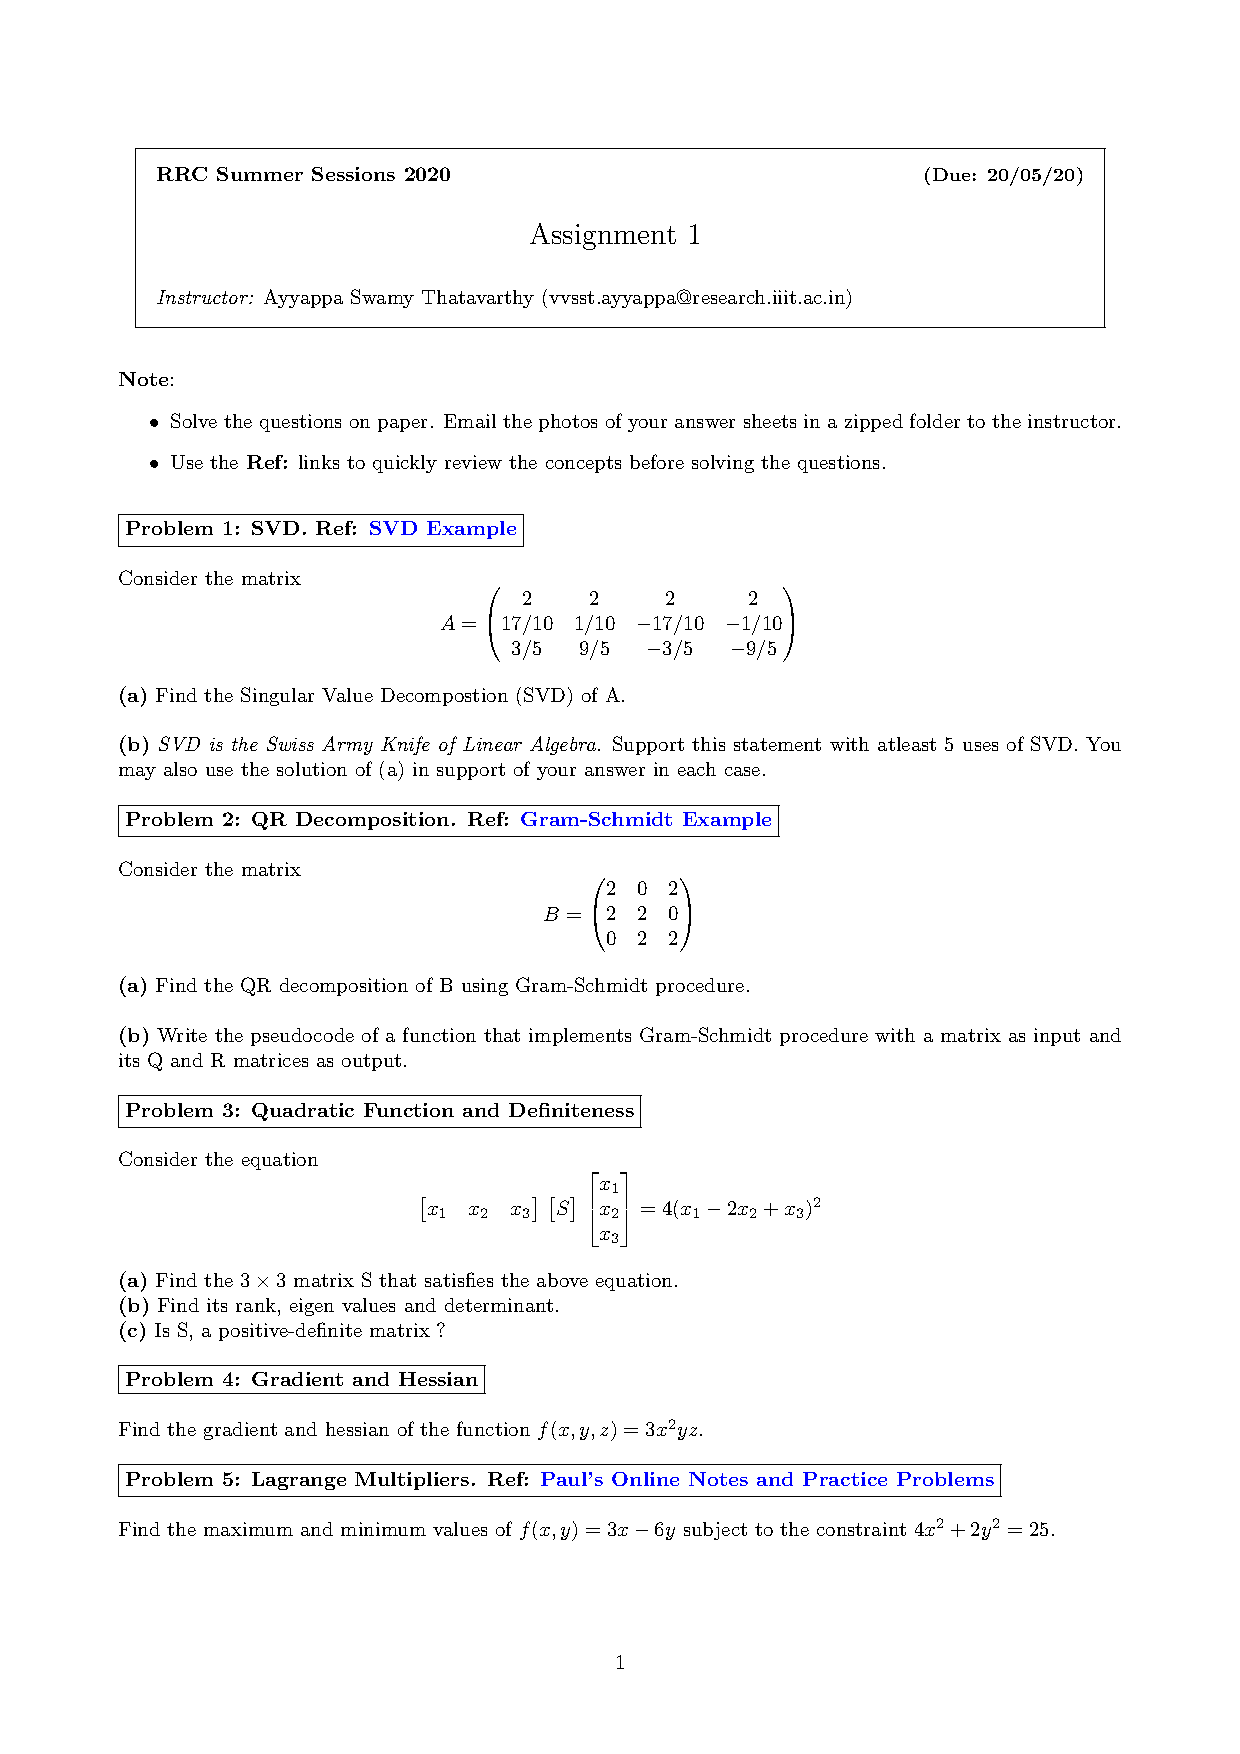
\includepdf[pages=-]{./Assignments/Assignment1.pdf}